\chapter{RESEARCH METHOD}
\label{chap:Chapter3}

The nature of neural network-based methods is to estimate the probability density of data, which requires normalization. In contrast, Diffusion models learn to estimate the gradients of data distribution \cite{song2021score} and do not require normalization over the entire dataset, resulting in better performance than neural network methods that do not use diffusion. Diffusion models can approximate data distributions even in low-density regions and generate highly detailed results.

This thesis builds upon the DiffuseStyleGesture model \cite{yang2022DiffuseStyleGestureplus}, with the main improvement being the integration of speech. Speech is transcribed into text, and the text is embedded to obtain textual semantic feature vectors, which are then used as conditioning vectors in the conditional diffusion process, as described in \autoref{subsec:feature_extraction}. In addition, in \textit{Stage 7. Rendering} (\autoref{fig:CommonStage}), Unity is used to visualize the generated gestures.

The main contributions of the thesis are presented in \autoref{sec:contribution}.

The thesis first describes the diffusion model in \autoref{sec:summary_diffusion}, followed by the proposed OHGesture model in \autoref{sec:ohgesture}.

\section{Basic Diffusion Model and Improvements}
\label{sec:summary_diffusion}

\begin{figure}[H]
	\centering
	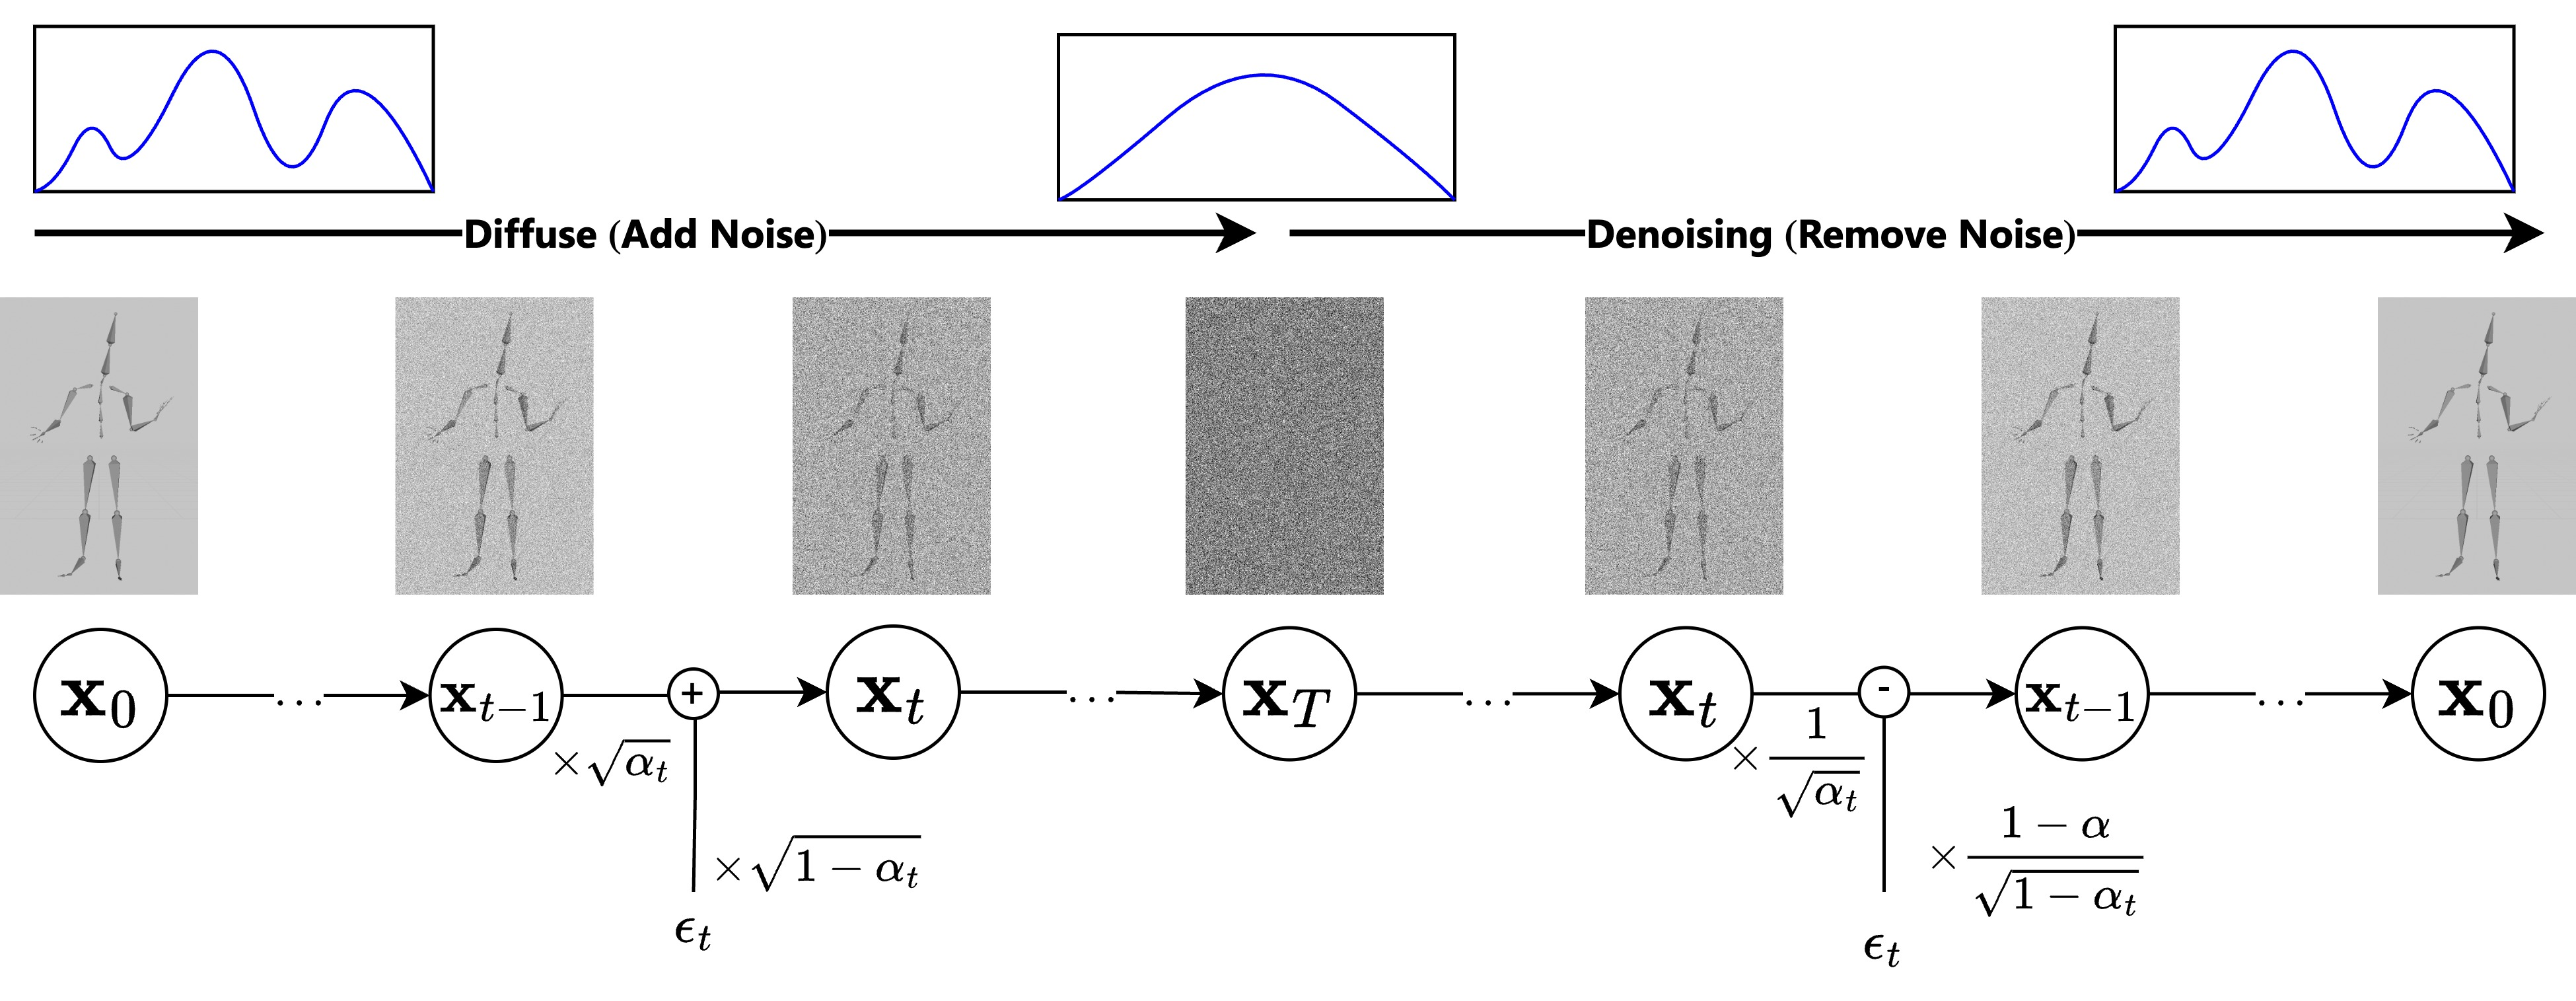
\includegraphics[width=\linewidth]{DiffuseAndDenoise}
	\caption{The \textbf{non-training} Diffusion and Denoising Process}
	\label{fig:DiffuseAndDenoise}
\end{figure}

In neural network methods like ResNet or InceptionNet, the goal is to learn the weight $\theta$ of a function $f_{\theta}(x)$ by minimizing a loss function $\mathcal{L}_\text{loss}$ between a label $y$ and its prediction $\hat{y}$. Once training is complete, the learned weight $\theta'$ can be used to predict a new sample $x'$ through $f_{\theta'}$ to obtain prediction $y'$.

Similarly to VAE, where the input matrix is encoded into a latent vector $z$ and then decoded back into a matrix of the original size, the diffusion model breaks the learning process into $T$ steps. At each step $t$, the forward diffusion process $q(\mathbf{x})$ from $1 \to T$ adds Gaussian noise $\epsilon_t \sim \mathcal{N}(\mathbf{0}, \mathbf{I})$, where $\mathbf{I}$ is the identity matrix of the standard Gaussian distribution with $\mathbb{E}[\epsilon] = 0$ and $\operatorname{Var}(\epsilon) = 1$.

The process of adding noise from left to right is called $q(\bx)$, while the denoising process from right to left is $p(\bx)$. Note that $\epsilon_t$ is randomly sampled at each step $t$, but once sampled, it is fixed. As illustrated in \autoref{fig:DiffuseAndDenoise}, if we add a noise $\epsilon_t$ during diffusion and subtract exactly the same noise during denoising, the result $\bx_0$ is \textbf{identical} to the original input.

However, during denoising, instead of subtracting the actual noise $\epsilon_t$, the model uses a function $f_{\theta}$ to \textbf{predict the added noise} during diffusion. Then, $\bx_T$ is iteratively denoised by subtracting the predicted noise to obtain $\hat{\bx}_{T-1}$, continuing until $\hat{\bx}_0$ is reached.

In the basic Diffusion model or Denoising Diffusion Probabilistic Models (DDPM \cite{ho2020denoising}), the denoising process goes from $T \to 1$, and the goal is to learn the weights $\theta$ of the noise prediction function $f_{\theta}$ (also denoted as $\epsilon_\theta$). After training, the learned weights $\theta'$ are used to predict the noise $\hat{\epsilon}$. Then, the noise is subtracted from the noisy image $\mathbf{x}_t$ to get $\mathbf{x}_{t-1}$, with additional noise $\mathbf{z} \sim \mathcal{N}(0, \mathbf{I})$ added to maintain gesture diversity. This process is repeated until reaching the final prediction $\hat{\bx}_0$.

\subsection{Forward Diffusion Process}

Given the input data $\mathbf{x}_0 \sim q(x)$ from the real dataset, at each step $t$, noise is added to $\mathbf{x}_{0}$ with the noise-to-signal ratio controlled by a factor $\beta$:

\begin{equation}
	\label{eq:addgaussian}
	\mathbf{x}_t = \sqrt{1 - \beta_t}\mathbf{x}_{t-1} + \sqrt{\beta_t} \boldsymbol{\epsilon}_{t-1}
\end{equation}

The forward process runs from $1 \to T$, with $\beta_t \in (0, 1)$ for each $t$.

Since a function of the form $f(x) = ax + b\epsilon$, with $\epsilon \sim \mathcal{N}(0, \mathbf{I})$, implies $f(x) \sim \mathcal{N}(ax, b^2)$, the forward process can be reformulated as:

\begin{equation}
	\label{eq:forward_diffusion_process}
	\begin{aligned}
		q(\mathbf{x}_t \vert \mathbf{x}_{t-1}) &= \mathcal{N}(\mathbf{x}_t; \sqrt{1 - \beta_t} \mathbf{x}_{t-1}, \beta_t\mathbf{I}) \quad \\
		q(\mathbf{x}_{1:T} \vert \mathbf{x}_0) &= \prod^T_{t=1} q(\mathbf{x}_t \vert \mathbf{x}_{t-1})
	\end{aligned}
\end{equation}

Here, $\sqrt{1 - \beta_t}$ gradually decreases the contribution of $\mathbf{x}_t$, while $\beta_t$ increases the noise component. Typically, $\beta_1 < \beta_2 < \dots < \beta_T$. As $T \to \infty$, $\mathbf{x}_T$ approaches a pure Gaussian distribution: $q(\mathbf{x}_T) = \mathcal{N}(0, \mathbf{I})$ \cite{weng2021diffusion}.

\begin{figure}[H]
	\centering
	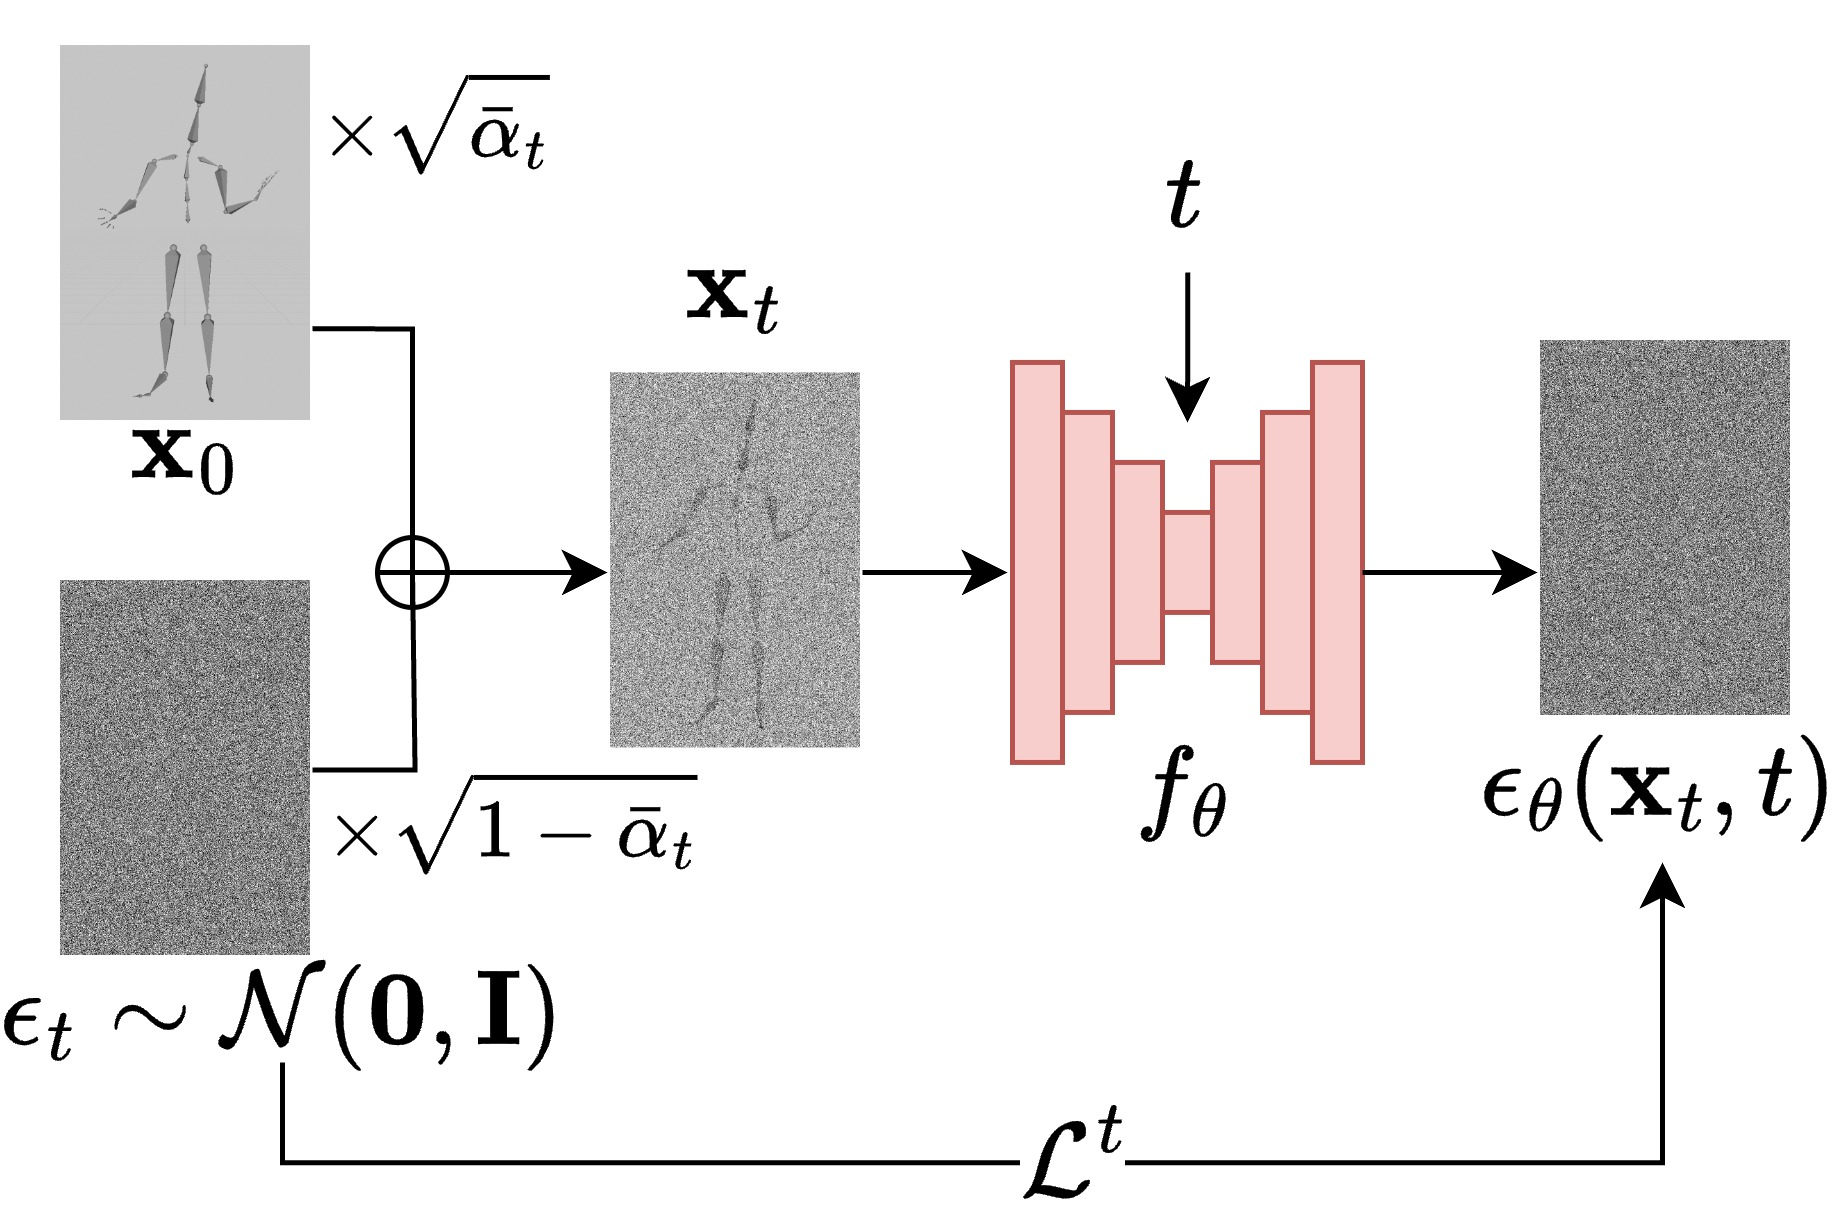
\includegraphics[height=160pt]{AlgorithmForwardDiffusion}
	\caption{Noise addition during training}
	\label{fig:AlgorithmForwardDiffusion}
\end{figure}

Since $\boldsymbol{\epsilon}_{t-1}, \boldsymbol{\epsilon}_{t-2}, \dots \sim \mathcal{N}(\mathbf{0}, \mathbf{I})$ and fixed for each $t$, $\bx_t$ can be computed directly from $\bx_0$. Define $\alpha_t = 1 - \beta_t$ and $\bar{\alpha}_t = \prod_{i=1}^t \alpha_i$, then \autoref{eq:addgaussian} becomes:

\begin{equation}
\begin{aligned}
	\boldsymbol{x}_t &= \sqrt{\bar{\alpha}_t} \boldsymbol{x}_0 + \sqrt{1 - \bar{\alpha}_t} \boldsymbol{\epsilon}_0 \\
	&\sim \mathcal{N}\left(\boldsymbol{x}_t; \sqrt{\bar{\alpha}_t} \boldsymbol{x}_0, \left(1 - \bar{\alpha}_t\right) \textbf{I}\right)
\end{aligned}
\label{eq:tracexzero}
\end{equation}

The evolution of $\sqrt{\alpha}$ and $\sqrt{1 - \alpha}$ over diffusion steps is shown in Appendix \autoref{appendix:Appendix1}.

\subsection{Denoising Process}
\label{subsection:denoising_process}

\begin{figure}[H]
	\centering
	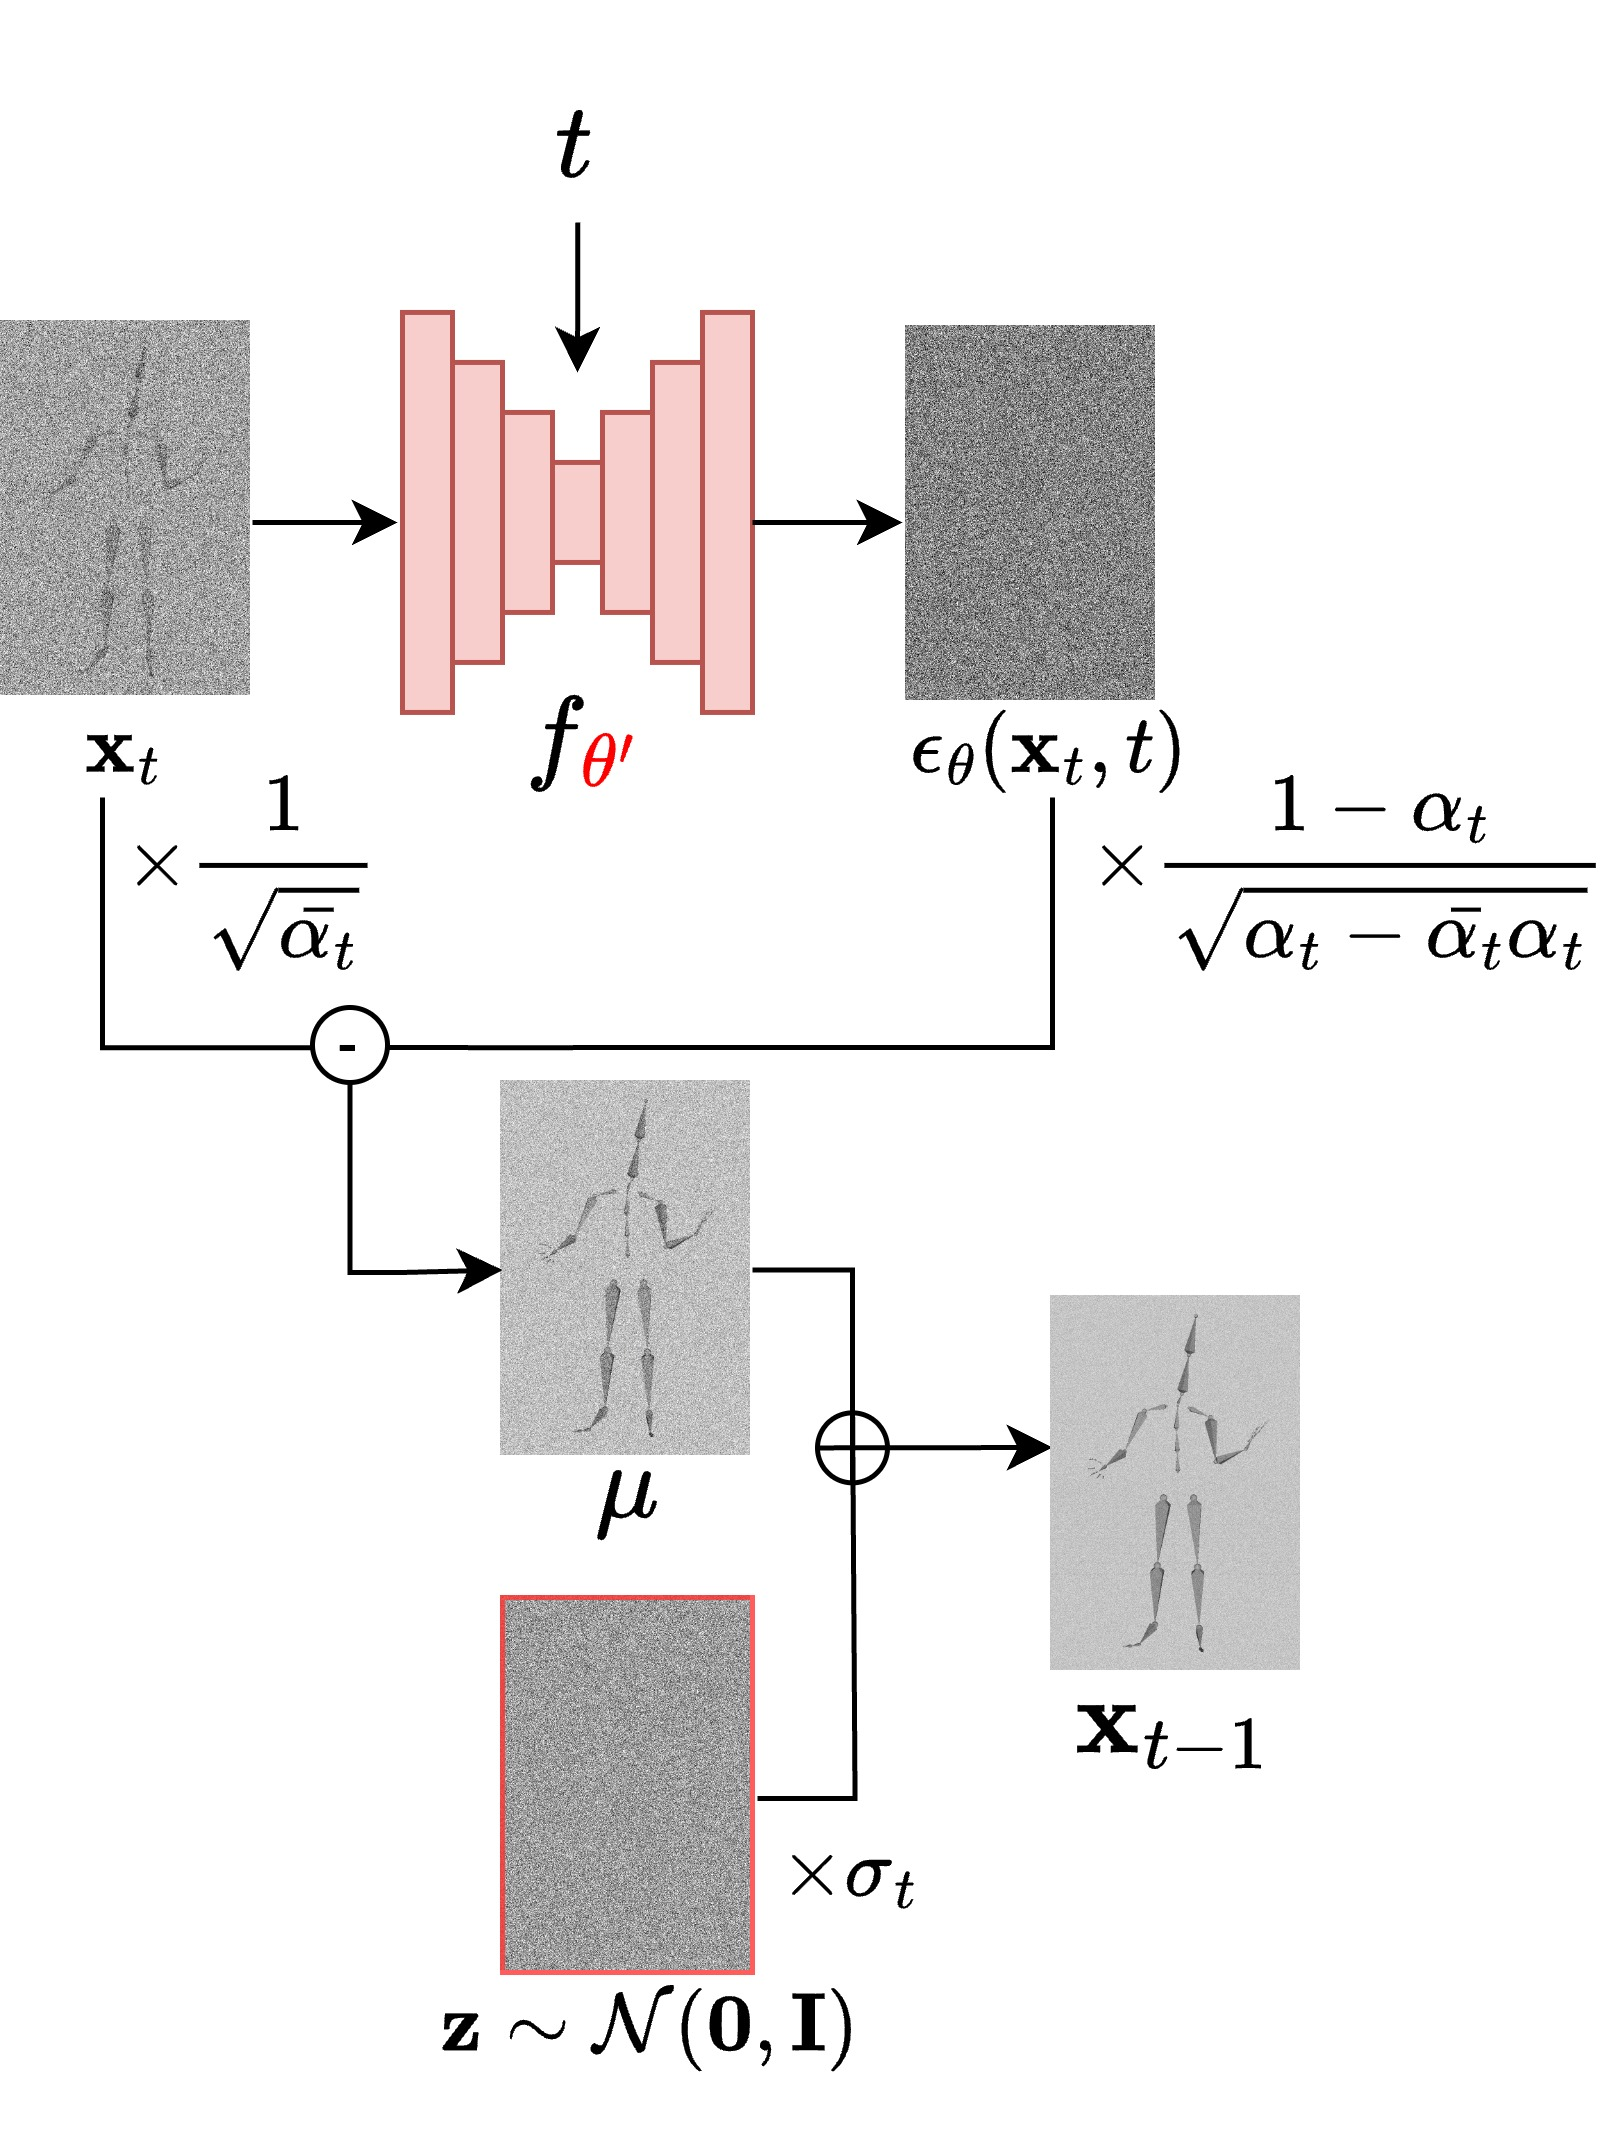
\includegraphics[height=280pt]{AlgorithmSamplingDiffusion}
	\caption{Denoising during inference}
	\label{fig:AlgorithmSamplingDiffusion}
	\vspace{-5pt}
\end{figure}

The denoising process $p_\theta(\mathbf{x}_{t-1} \vert \mathbf{x}_t)$ starts from $\bx_T \sim \mathcal{N}(\mathbf{0}, \mathbf{I})$. A neural network $f_{\theta}(\bx_t, t)$ is used to predict the noise $\hat{\epsilon}_t = f_{\theta}(\bx_t, t)$.

The denoising distribution has mean and variance:

\begin{equation}
	\label{eq:denoising_process}
	\begin{aligned}
		p_\theta(\mathbf{x}_{0:T})
		&= p(\mathbf{x}_T) \prod^T_{t=1} p_\theta(\mathbf{x}_{t-1} \vert \mathbf{x}_t) \\
		p_\theta(\mathbf{x}_{t-1} \vert \mathbf{x}_t) &= \mathcal{N}(\mathbf{x}_{t-1};  \boldsymbol{\mu}_\theta(\mathbf{x}_t, t), \boldsymbol{\Sigma}_\theta(\mathbf{x}_t, t))
	\end{aligned}
\end{equation}

where $\boldsymbol{\mu}_\theta(\mathbf{x}_t, t) = {\frac{1}{\sqrt{\alpha_t}} \left( \mathbf{x}_t - \frac{1 - \alpha_t}{\sqrt{1 - \bar{\alpha}_t}}  f_\theta(\mathbf{x}_t, t) \right)}$.

\subsection{Training Process in the Basic Diffusion Model}

\begin{figure}[H]
	\centering
	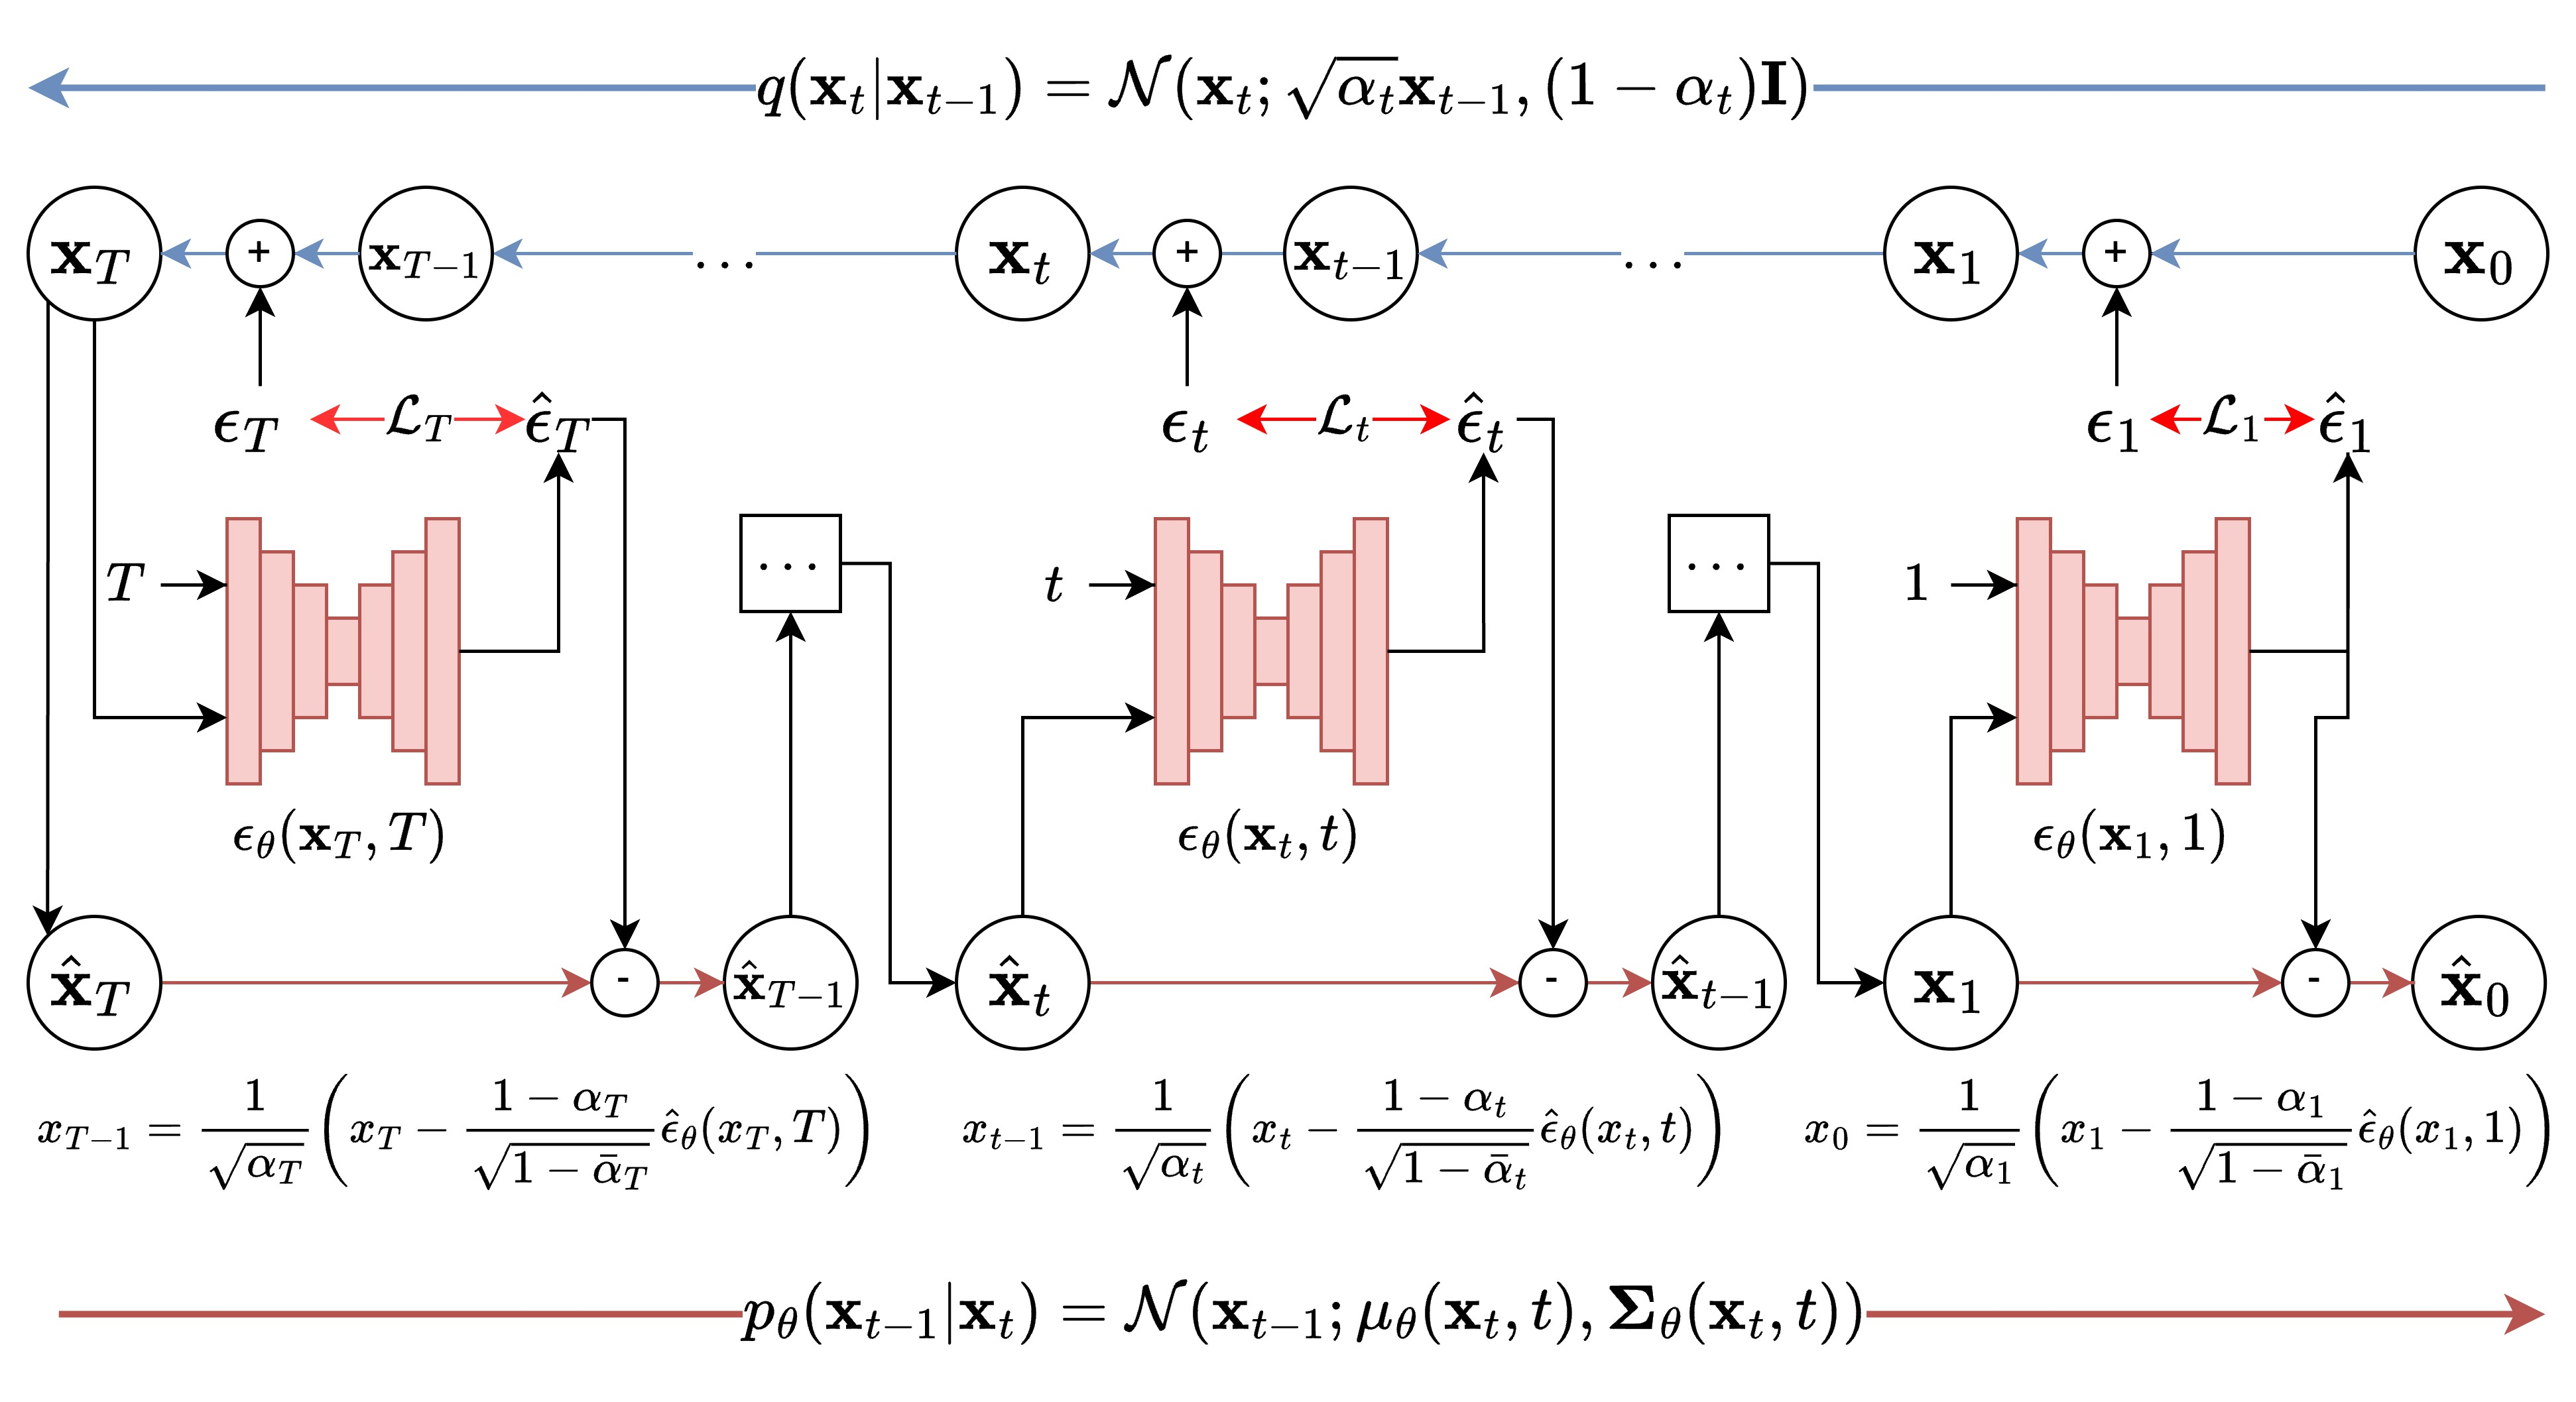
\includegraphics[width=\linewidth]{DDPMTraining}
	\caption{Basic diffusion model}
	\label{fig:basic_diffusion}
	\vspace{-5pt}
\end{figure}

The diffusion model learns the parameters $\theta$ of the noise prediction function $f_{\theta}(\bx_t, t)$ (or $\epsilon_\theta$). During denoising, we minimize the loss between the predicted noise $\boldsymbol{\epsilon}_\theta(\bx_t, t)$ and actual noise $\boldsymbol{\epsilon}_t$ at each step $t$:

\begin{equation}
	\label{eq:diffusion_loss}
	\begin{aligned}
		\mathcal{L}^t
		&= \mathbb{E}_{t \sim [1, T], \bx_0, \boldsymbol{\epsilon}_t} \left[\|\boldsymbol{\epsilon}_t - \boldsymbol{\epsilon}_\theta(\bx_t, t)\|^2 \right] \\
		&= \mathbb{E}_{t \sim [1, T], \bx_0, \boldsymbol{\epsilon}_t} \left[\|\boldsymbol{\epsilon}_t - \boldsymbol{\epsilon}_\theta(\sqrt{\bar{\alpha}_t}\bx_0 + \sqrt{1 - \bar{\alpha}_t}\boldsymbol{\epsilon}_t, t)\|^2 \right]
	\end{aligned}
\end{equation}

The total loss is $\mathcal{L} = \sum_{t=1}^T \mathcal{L}^t$.

Here, $f_{\theta}(x_t, t)$ or $\epsilon_\theta$ is a U-Net model used to encode and decode the data for noise prediction. The computation process is illustrated in \autoref{fig:basic_diffusion}.

\begin{algorithm}[H]
	\setlength{\baselineskip}{10pt}
	\begin{enumerate}
		\vspace{5pt}
		\item Precompute $\sqrt{\alpha_t}$, $\sqrt{1 - \alpha_t}$, and $\sqrt{\bar{\alpha}_t}$ for $t = 1 \rightarrow T$. Define noise schedule $\{\alpha_t \in (0, 1)\}_{t=1}^T$ with $\alpha_1 < \alpha_2 < \dots < \alpha_T$.
		
		\item Sample label $\bx_0$ from the normalized data distribution.
		
		\item Generate random noise $\boldsymbol{\epsilon}_t$ for each step $t = 1 \rightarrow T$, where $\boldsymbol{\epsilon}_t \sim \mathcal{N}(\mathbf{0}, \mathbf{I})$.
		
		\item Apply forward diffusion to get $\bx_t$:
		$$
		\bx_t = \sqrt{\bar{\alpha}_t} \bx_0 + \sqrt{1 - \bar{\alpha}_t} \boldsymbol{\epsilon}_t
		$$
		
		\item Randomly select $t \in [1, T]$.
		
		\item Feed $\bx_t$ and $t$ into the model to predict noise: $\hat{\boldsymbol{\epsilon}} = \boldsymbol{\epsilon}_\theta(\bx_t, t)$.
		
		\item Compute the gradient:
		$$
		\grad_{\theta_t} \left\| \boldsymbol{\epsilon}_t - \boldsymbol{\epsilon}_\theta(\bx_t, t) \right\|^2
		$$
		
		And loss:
		$$
		\mathcal{L}^t = \mathbb{E}_{t, \bx_0, \boldsymbol{\epsilon}_t} \left[ \|\boldsymbol{\epsilon}_t - \boldsymbol{\epsilon}_\theta(\sqrt{\bar{\alpha}_t} \bx_0 + \sqrt{1 - \bar{\alpha}_t} \boldsymbol{\epsilon}_t, t)\|^2 \right]
		$$
		
		\item Repeat step 6 until convergence to obtain optimal weights $\theta'$.
	\end{enumerate}
	\caption{DDPM Training Algorithm}
	\label{alg:TrainingDDPM}
\end{algorithm}

\subsection{Basic Sampling Process in Diffusion Models}

\begin{figure*}
	\centering
	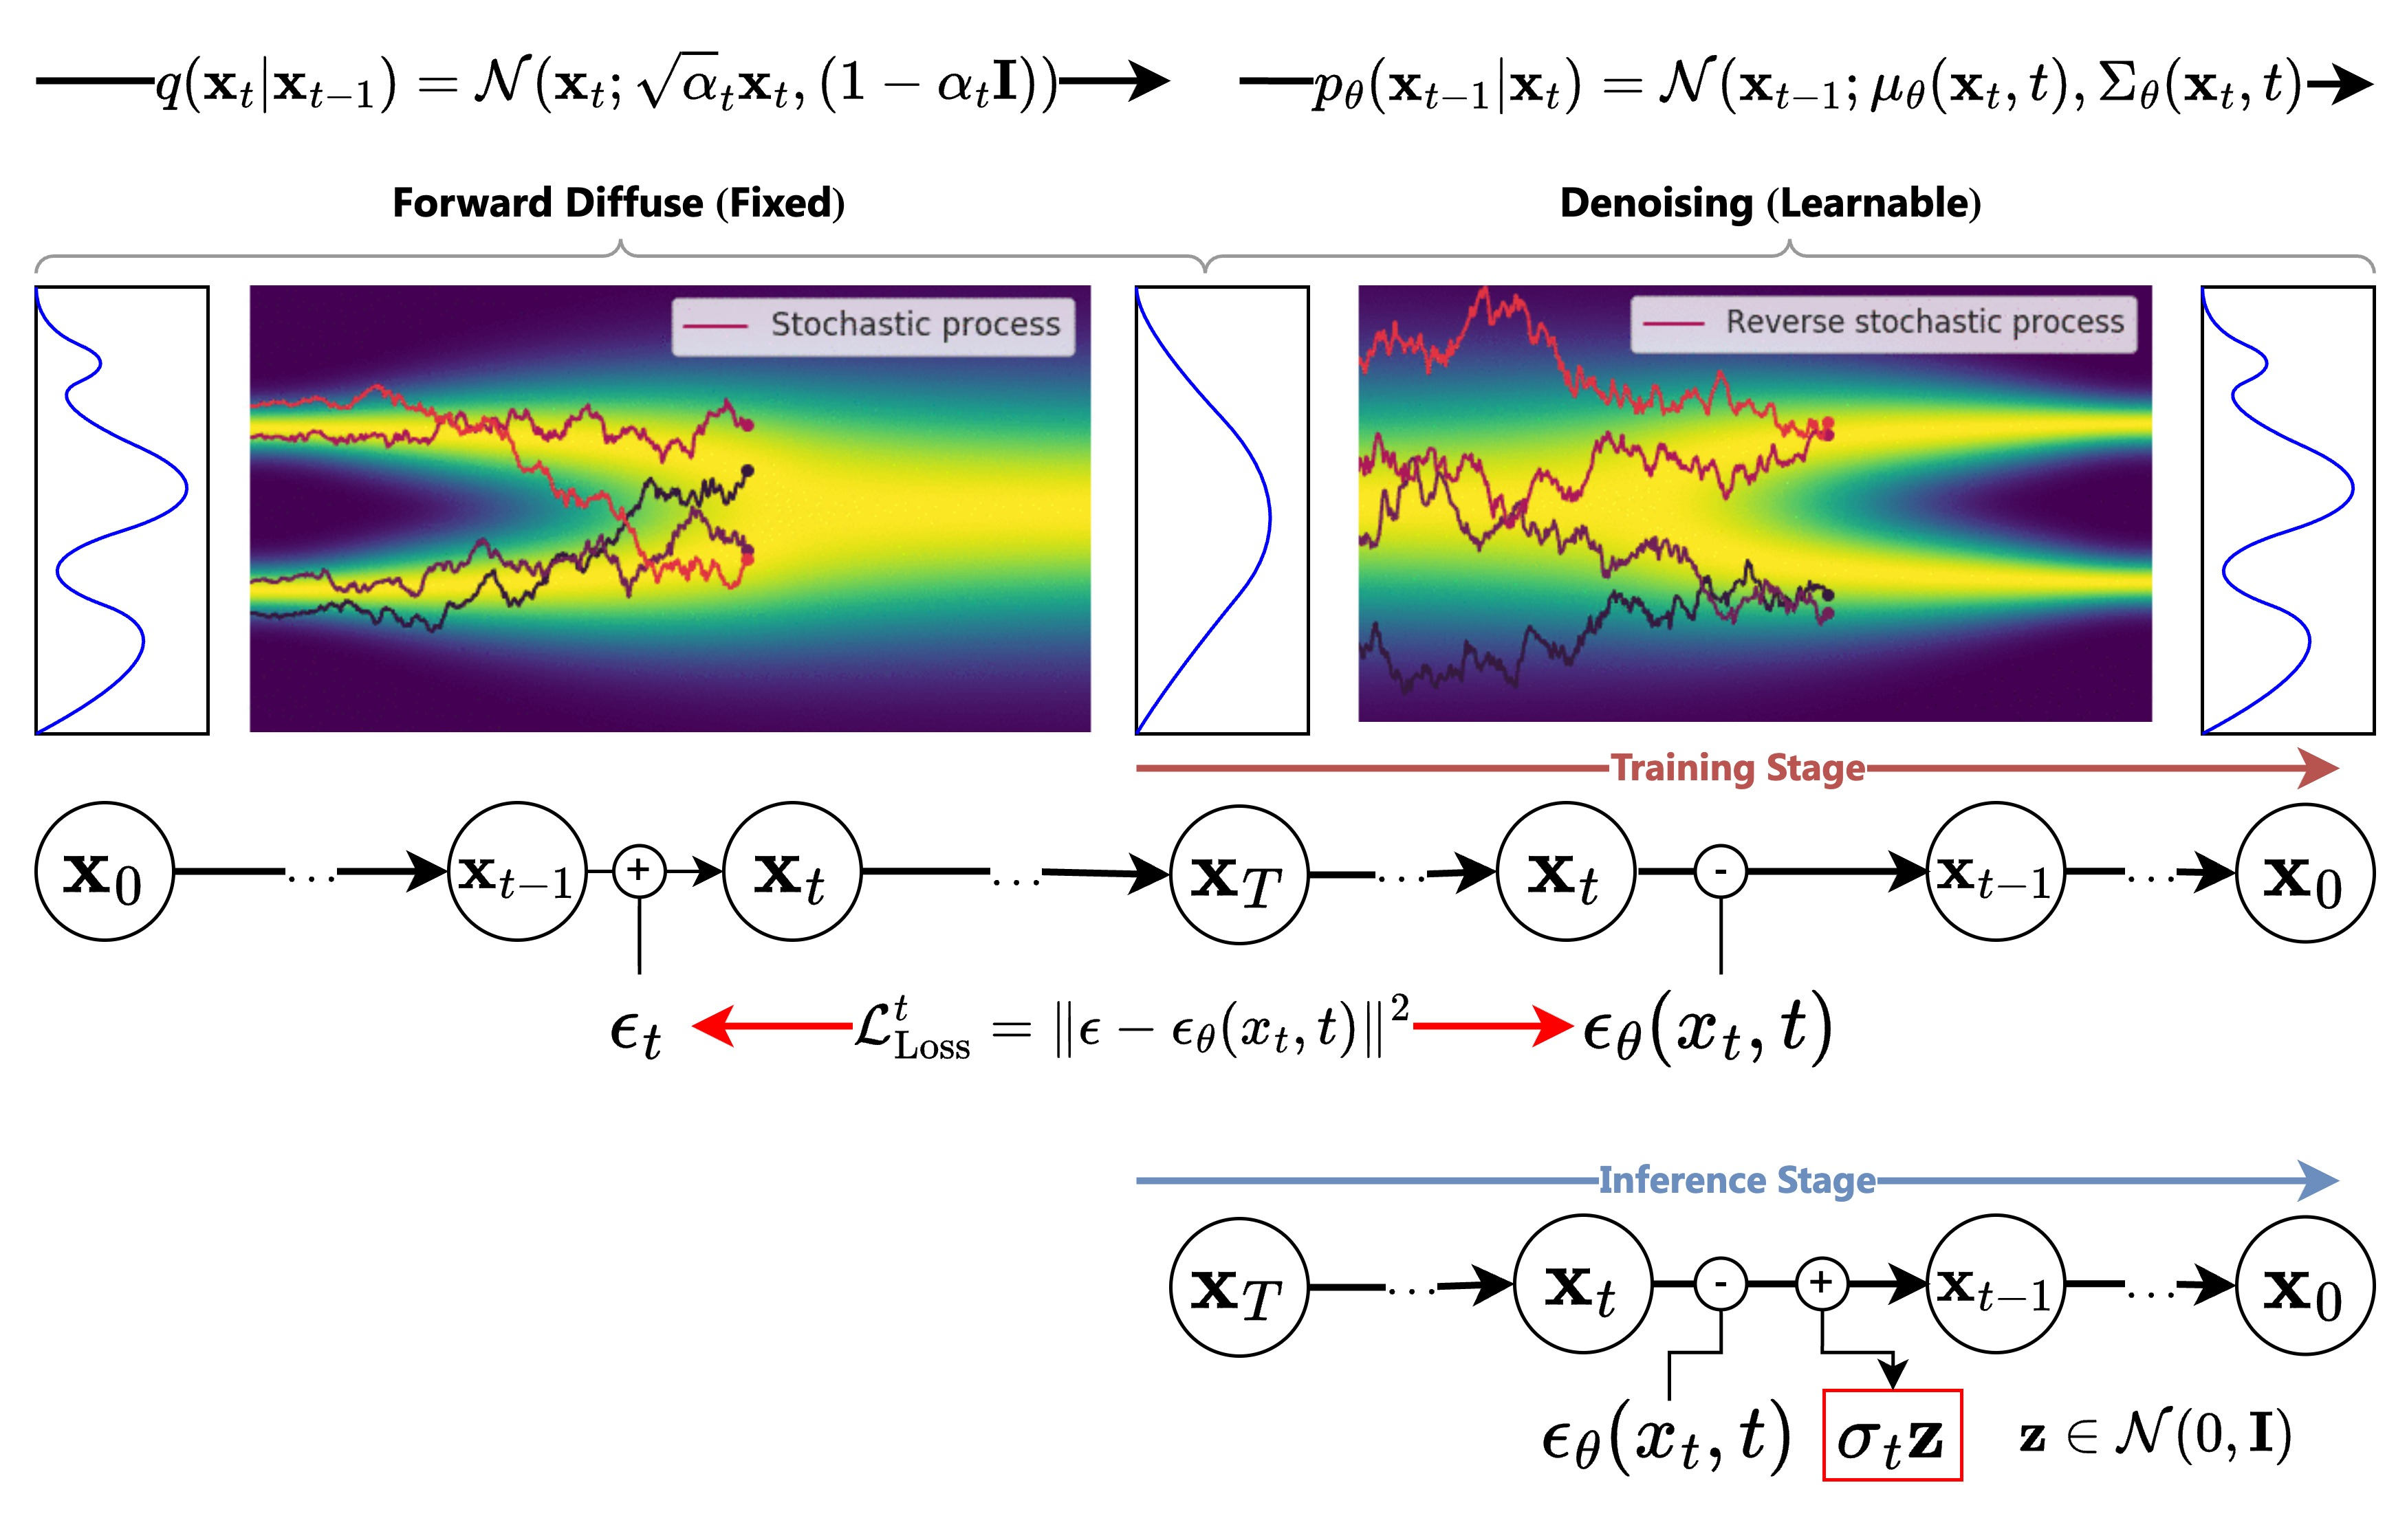
\includegraphics[width=\linewidth]{TrainingAndSamplingStandard}
	\caption{Training and Sampling process in a standard Diffusion model}
	\label{fig:GaussianDrift}
\end{figure*}

After obtaining the weights $\theta'$, the denoising function is used to denoise from noise $\bx_T \sim \mathcal{N} (\mathbf{0}, \mathbf{I})$.  
The transformation from pure noise $\bx_{T}$ to the prediction $\hat{\bx_0}$ is as follows:

\begin{equation}
	\label{eq:adddenoising}
	\bx_{t-1} = \frac{1}{\sqrt{\alpha_t}} \left( \bx_t - \frac{1- \alpha_t}{\sqrt{1 - \bar{\alpha}_t}} f_{\theta'}(\bx_t, t) \right) + \sqrt{1 - \alpha_t} \tilde{\epsilon}_t
\end{equation}

Note that $\epsilon_t$ is fixed and randomly generated noise created before the training process, and reused during the forward diffusion process \autoref{subsection:denoising_process} in formula \autoref{eq:addgaussian}. As shown in \autoref{fig:GaussianDrift}, the error $\epsilon_t$ corresponds to the noise at each step $t$, and the loss function $\mathcal{L}^{t}$ is computed per time step $t$.

Following the training process, the DDPM sampling algorithm begins from pure noise, i.e., $\mathbf{x}_T \sim \mathcal{N}(0, \mathbf{I})$, where the initial data is entirely noise. The values $\sqrt{\alpha_t}$, $\sqrt{1 - \alpha_t}$, and $\sqrt{\bar{\alpha}_t}$, obtained from the training phase, are used during sampling to reconstruct the original data $\mathbf{x}_0$. The next step is to compute the noise adjustment coefficient $\sigma_t$, based on the noise schedule $\alpha_t$ defined during training. These values influence the amount of noise added in the reverse sampling process.

The sampling process (\autoref{alg:samplingddpm}) proceeds from step $T$ down to $1$, and at each step, a random noise $\mathbf{z} \sim \mathcal{N}(0, \mathbf{I})$ is generated and added to the predicted result. At each step $t$, the model predicts the noise $\boldsymbol{\epsilon}_{\theta'}$ based on the noisy data $\mathbf{x}_t$ and time step $t$, then uses this prediction to compute the value $\mu$, an estimate of $\mathbf{x}_0$. Finally, a noise term $\sigma_t \mathbf{z}$ is added to $\mu$ to obtain $\hat{\mathbf{x}}_{t-1}$, the noisy data at step $t-1$. This process continues until $t = 1$, at which point $\hat{\mathbf{x}}_0$ — the final prediction of the original data — is obtained through denoising.

\begin{algorithm}[H]
	\caption{Sampling algorithm in DDPM}
	\label{alg:samplingddpm}
	\setlength{\baselineskip}{10pt}
	\begin{enumerate}
		\item Start with noise: $\mathbf{x}_T \sim \mathcal{N}(0, \mathbf{I})$.
		
		\item Retrieve values $\sqrt{\alpha_t}$, $\sqrt{1 - \alpha_t}$, and $\sqrt{\bar{\alpha}_t}$ from the training process.
		
		\item Compute the noise adjustment coefficient $\sigma_t$ from $\alpha_t$ at each step $t: 1 \rightarrow T$:
		\[
		\sigma_t = \sqrt{\frac{1 - \bar{\alpha}_{t-1}}{1 - \bar{\alpha}_t} (1 - \alpha_t)}
		\]
		
		\item For each $t$, iterate \textbf{sequentially} from $[T, \dots, 1]$.
		
		\item Generate random noise $\mathbf{z} \sim \mathcal{N}(0, \mathbf{I})$.
		
		\item Feed $\mathbf{x}_t$ into the model to infer noise: $\boldsymbol{\epsilon}_{\theta'} = \boldsymbol{\epsilon}_{\theta'}(\mathbf{x}_t, t)$.
		
		\item Use the predicted noise to subtract from $\mathbf{x}_t$ at step $t$:
		\[
		\mu = \frac{1}{\sqrt{\alpha_t}} \left( \mathbf{x}_t - \frac{1 - \alpha_t}{\sqrt{1 - \bar{\alpha}_t}} \boldsymbol{\epsilon}_{\theta'}(\mathbf{x}_t, t) \right)
		\]
		
		\item Add noise: $\hat{\mathbf{x}}_{t-1} = \mu + \sigma_t \mathbf{z}$.
		
		\item When $t = 1$, obtain $\hat{\mathbf{x}}_0$ from the denoising process.
	\end{enumerate}
\end{algorithm}

The most important aspect of the denoising sampling process is to add a noise term $\mathbf{z} \in \mathcal{N}(0, \mathbf{I})$, with $\mathbf{z}$ sequentially added at each step $t$ using the scaling factor $\sigma_t$. The goal of noise $\epsilon$ is to shape the marginal noise distribution so that model $f_\theta$ (or $\epsilon_{\theta}$) can learn to denoise, whereas $\mathbf{z}$ is used to increase diversity in generation and improve stability during sampling. The decay of $\sigma_t$ is detailed in Appendix \autoref{appendix:Appendix1:NoiseScale}.

\subsection{Improved Diffusion Model with $\bx_0$ Prediction Instead of $\epsilon_t$}
\label{subsec:X0Objective}

Based on \autoref{eq:tracexzero}, it is clear that given $\bx_t$, we can infer $\bx_0$. Conversely, given $\bx_0$, we can explicitly infer $\bx_t$ for any $t$ by adding the noise $\epsilon_t$ from the forward diffusion process.

From this observation, the authors in \cite{nichol2021improved} proposed an improvement to DDPM: instead of using the neural network $f_{\theta}(\bx_t, t)$ to predict $\epsilon_t$ as in \autoref{fig:basic_diffusion}, the function $f_{\theta}(\bx_t, t)$ is repurposed to directly predict $\bx_0$, after which noise is added using \autoref{eq:tracexzero}.

\begin{figure}[H]
	\captionsetup{skip=2pt}
	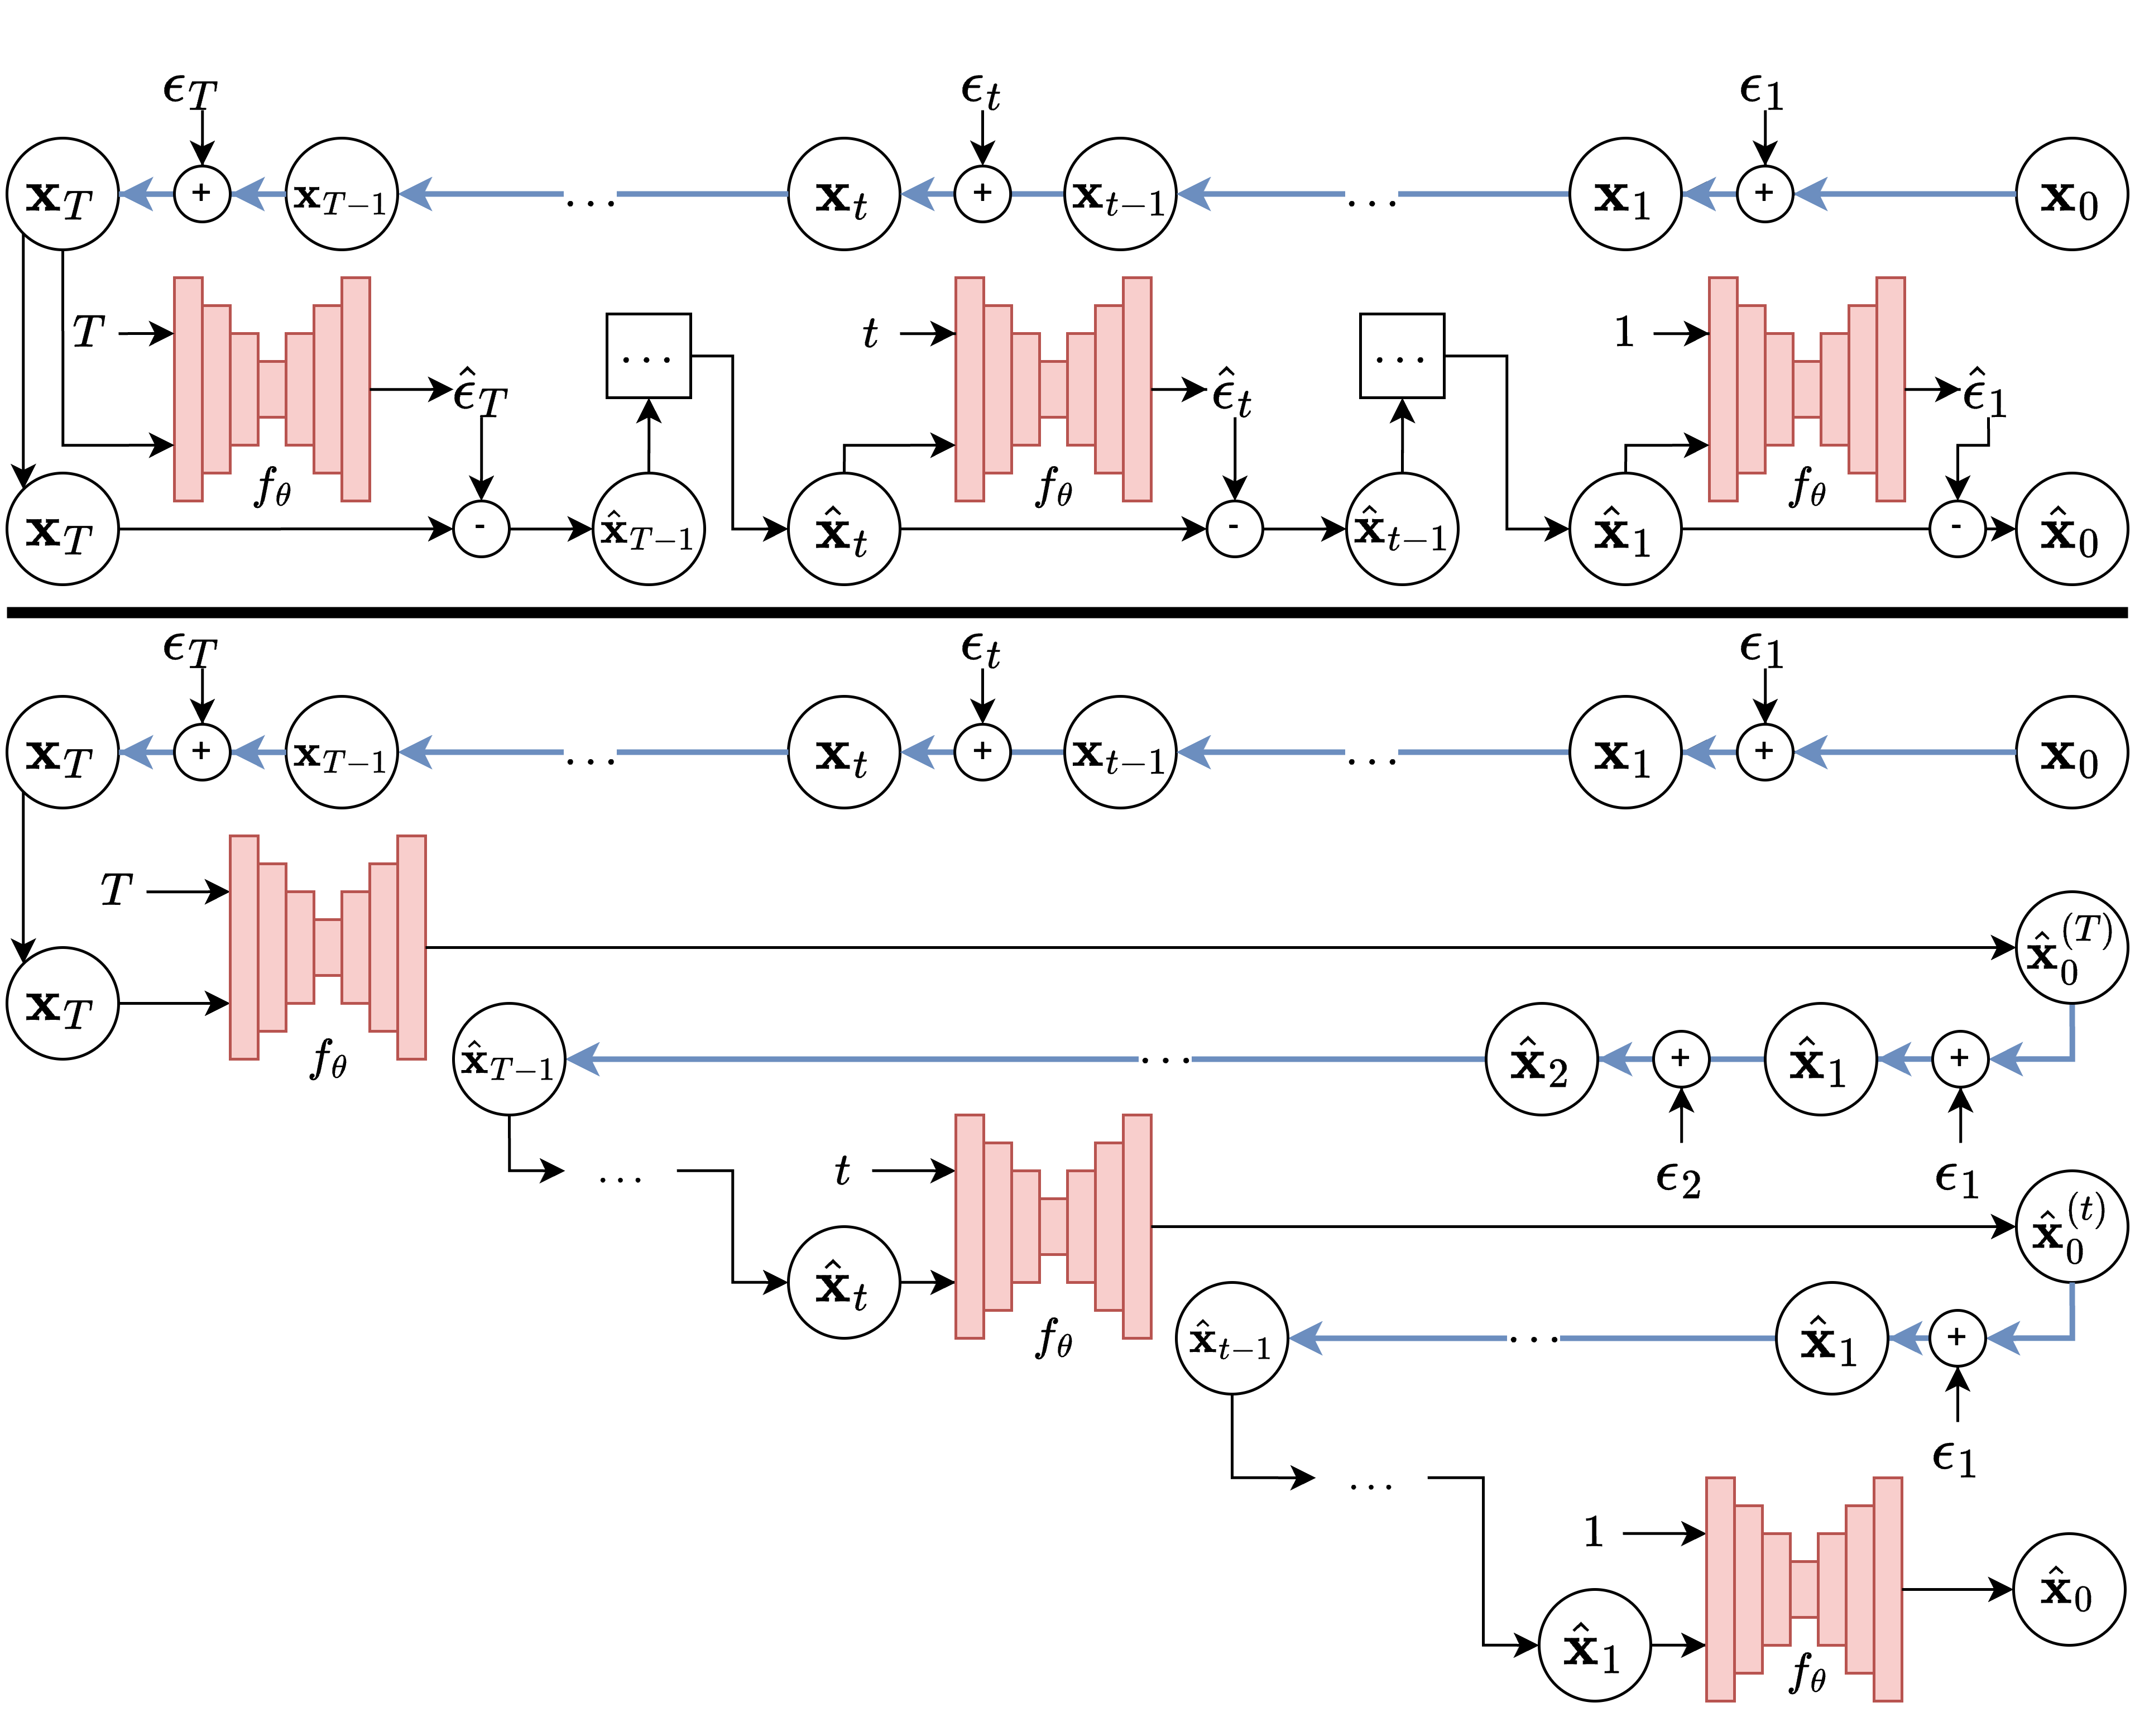
\includegraphics[width=\linewidth]{X0Objective}
	\caption{Comparison between $\epsilon$ objective (top) and $\bx_0$ objective (bottom)}
	\label{fig:X0Objective}
\end{figure}

As shown in \autoref{fig:X0Objective}, we start with forward diffusion from $t: 1 \rightarrow T$ to obtain $\bx_T \sim \mathcal{N} (0, \mathbf{I})$. After acquiring $\bx_T$, we feed it into $f_{\theta}$ to predict $\hat{\bx}_0$, and from $\hat{\bx}_0$ we add noise to obtain $\hat{\bx}_{t-1}$. This continues until $t = 1$, when $\hat{\bx}_0$ is ultimately obtained. We can compare the two methods as follows:

\begin{itemize}
	\item \textbf{$\epsilon$ objective}: the model predicts the noise. Begin with forward noise injection to get $\bx_T$, then use $\bx_T \in \mathcal{N}(0, \mathbf{I})$ as input for denoising. During denoising, the model predicts the noise $\hat{\epsilon}_t$ added in the forward step, i.e., $\epsilon_t$, and minimizes the error between the predicted and actual forward noise.
	\item \textbf{$\bx_0$ objective}: similarly, the model applies forward diffusion to get $\bx_T$, then uses $\bx_T \in \mathcal{N}(0, \mathbf{I})$ for denoising. The model directly predicts $\bx_0$, then reintroduces noise to compute $\bx_{t-1}$, and continues using $\bx_{t-1}$ as input to predict $\bx_0$ again.
\end{itemize}

\subsection{Conditional Diffusion Models}
\label{subsec:DiffusionCondition}

To control the generation process under different conditions, generation must be conditioned on $c$—that is, we aim to model $p(\bx | c)$ given condition $c$. The authors in \cite{dhariwal2021diffusion} proposed using a separate function $f_{\phi}$ to train the conditional component. However, this approach presents difficulties when the conditions change, and combining or updating weights in a separate model is challenging for scalability.

\begin{figure}[H]
	\captionsetup{skip=20pt}
	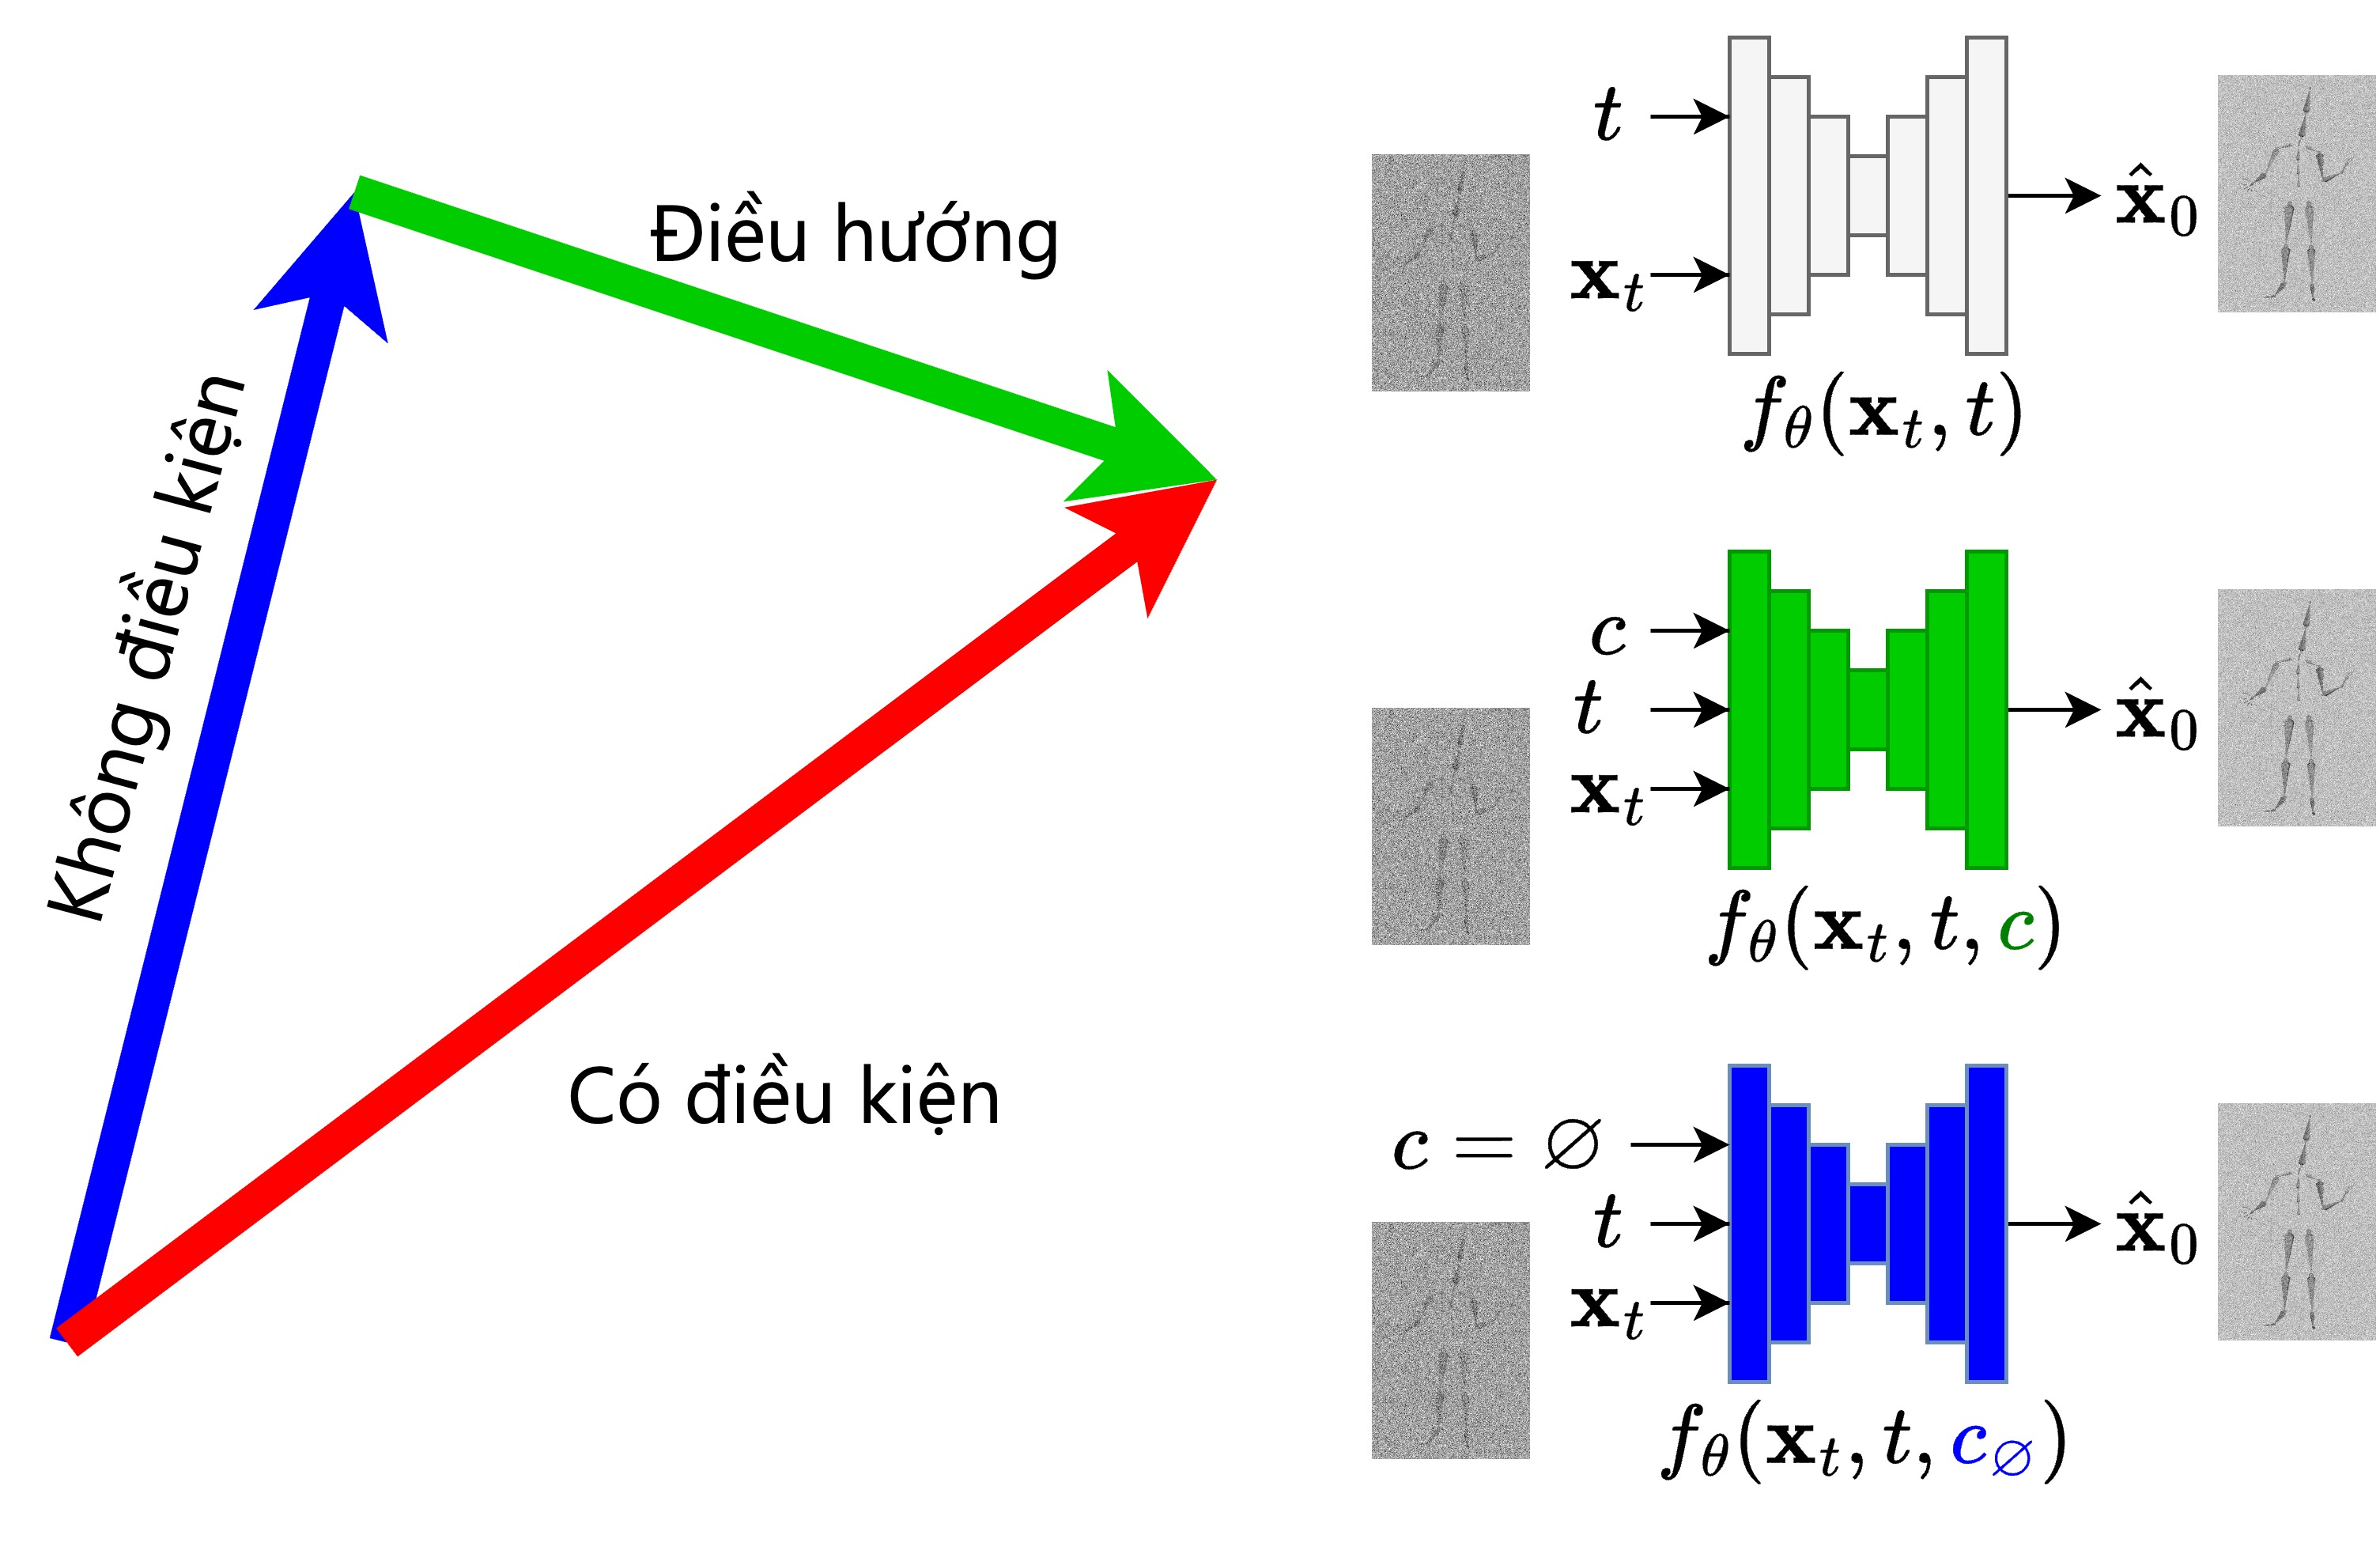
\includegraphics[width=0.9\linewidth]{AdversarialGradient}
	\caption{Conditional Diffusion via Guidance Vector}
	\label{fig:AdversarialGradient}
\end{figure}

As shown in \autoref{fig:GaussianDrift}, to allow inference to generate different $\bx_0$ samples controllably based on condition $c$, a guidance term must be added at each step $t$. The authors proposed Classifier-Free Diffusion Guidance \cite{ho2022classifier}, in which the result $\bx_0$ is updated by combining the conditional and unconditional outputs:

\begin{equation}
{\color{red}{\hat{\mathbf{x}}}}_{0 \gamma, \color{green}{c}, \color{blue}{c_{\varnothing}}}=\gamma \cdot f_{\theta} \left(\mathbf{x}_{t}, t, {\color{green}{c}} \right)+(1-\gamma) \cdot f_{\theta} \left(\mathbf{x}_{t}, t, {\color{blue}{c_{\varnothing}}} \right)
\end{equation}

Here, $c$ is the condition, $c_{\varnothing}$ is the null (empty) condition, and the conditional generation is controlled by the parameter $\gamma$: the larger $\gamma$ is, the closer the result aligns with condition $c$; conversely, a smaller $\gamma$ leads to a result closer to the unconditional output.

As illustrated in \autoref{fig:AdversarialGradient}, the top function $f_{\theta}$ is unconditional, the middle one is conditional diffusion, and the bottom one is diffusion under an empty condition.
